% ===================================================================
\begin{ex}
	Năng lượng gió ở Việt Nam có tiềm năng phát triển năng rất lớn. Trong thời gian tới, điện gió tiếp tục được kỳ vọng là một trong những nguồn năng lượng tái tạo chủ lực của Việt Nam. Chính phủ Việt Nam đã đặt mục tiêu đến năm 2030, tổng công suất lắp đặt điện gió đạt $\SI{12000}{\mega\watt}$. Hình bên dưới là mô hình đơn giản của mạng lưới cung cấp điện gió. Cho rằng roto máy phát điện quay với tốc độ góc không đổi $\omega$, các máy biến áp lý tưởng. Tổng trở trên đường dây truyền tải được đơn giản hóa thành điện trở không đổi $R_0$. Khi điện áp nơi tiêu thụ được nối với tải $R$ thì công suất tiêu thụ điện trên $R_0$ là $\calP$. Bỏ qua các hao phí khác.
	\begin{center}
		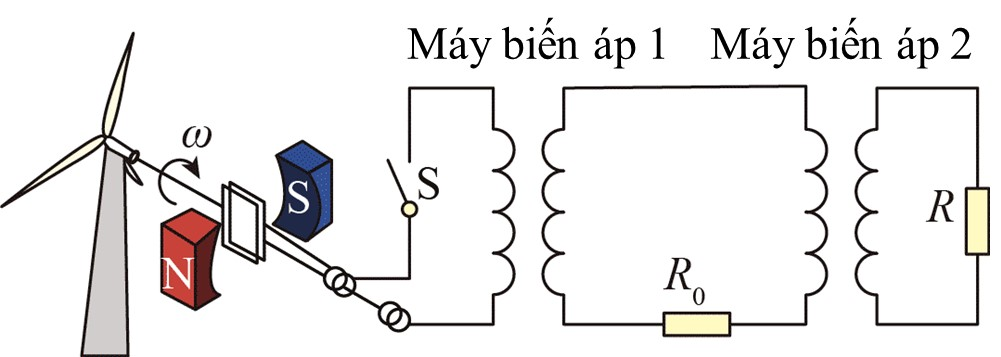
\includegraphics[scale=0.6]{../figs/THPTQG-002-2}
	\end{center}
	\choiceTF
	{\True Máy biến áp 1 là máy tăng áp và máy biến áp 2 là máy hạ áp}
	{\True Nếu gió thổi mạnh và làm tuabin quay với tốc độ gấp đôi thì công suất tiêu thụ điện trên $R_0$ tăng gấp 4 lần}
	{Nếu số vòng dây cuộn thứ cấp của máy biến áp 1 tăng gấp đôi thì công suất tiêu thụ điện trên $R_0$ là $8\calP$}
	{Nếu chiều dài đường dây truyền tải tăng gấp đôi thì công suất tiêu thụ điện trên $R_0$ tăng 4 lần}
	\loigiai{
	\begin{itemchoice}
		\itemch Đúng.
		\itemch Đúng.\\
		Gọi: 
		\begin{itemize}
			\item $k$ là hệ số giảm áp của máy biến áp 2;
			\item $k'$ là hệ số tăng áp của máy biến áp 1.
		\end{itemize} Có thể vẽ lại sơ đồ mạch điện:
		\begin{center}
			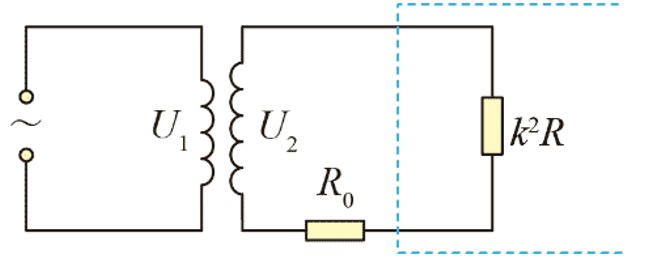
\includegraphics[scale=0.7]{../figs/THPTQG-002-3}
		\end{center}
		Cường độ dòng điện hiệu dụng qua $R_0$:
		$$I_2=\dfrac{U_2}{R_0+k^2R}=\dfrac{k'NBS\omega}{\sqrt{2}\cdot\left(R_0+k^2R\right)}.$$
		Khi $\omega$ tăng 2 lần thì $I_2$ tăng 2 lần $\Rightarrow \calP$ tăng 4 lần.
		\itemch Sai. Số vòng cuộn thứ cấp của máy biến áp tăng áp tăng gấp đôi, hiệu điện thế ở hai đầu cuộn thứ cấp tăng gấp đôi, dòng điện trên đường dây tăng gấp đôi nên công suất điện tiêu thụ trên $R_0$ tăng gấp 4 lần $\calP$.
		\itemch Sai. $I'_2=\dfrac{k'NBS\omega}{\sqrt{2}\cdot\left(2R_0+k^2R\right)}\Rightarrow \calP'=I'^2_2\cdot2R_0\neq 4\calP.$
	\end{itemchoice}
	}
\end{ex}
% ===============================================================
\textit{Dữ kiện dùng chung cho câu hỏi 1 và 2:}\\
\immini{Hình a là một dụng cụ rót rượu bằng đồng từ thời Chiến Quốc, được khai quật tại Sơn Đông của Trung Quốc. Hình b là sơ đồ mô phỏng đơn giản dụng cụ trên với một cán dài hình trụ rỗng và bầu chứa rượu dạng hình trụ ở bên dưới. Cán được nút kín ở một đầu và có tiết diện $S_1=\SI{1.0}{\centi\meter^2}$, chiều dài $H=\SI{100.0}{\centi\meter}$ với một lỗ nhỏ A trên thành bên. Bình chứa có tiết diện đáy $S_2=\SI{90}{\centi\meter^2}$, chiều cao $h=\SI{20.0}{\centi\meter}$ và một lỗ nhỏ B ở đáy bình. Nhúng dụng cụ rót rượu theo phương thẳng đứng vào thùng chất rượu, rượu đi vào từ lỗ B và không khí thoát ra ngoài từ lỗ A. Khi mức chất lỏng bên trong và bên ngoài bằng nhau, phần chiều dài của cán nhúng ngập vào trong rượu là $x$ thì chặn lỗ A rồi từ từ nhấc dụng cụ rót theo phương thẳng đứng ra khỏi thùng rượu. }
{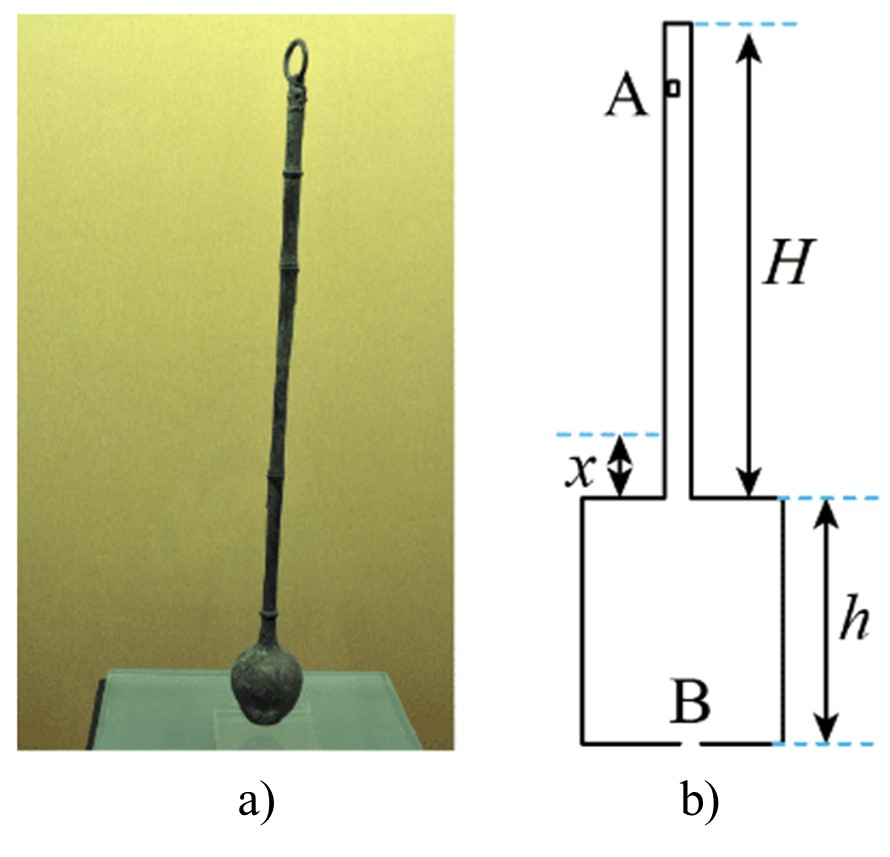
\includegraphics[scale=0.5]{../figs/THPTQG-002-1}}
Biết khối lượng riêng của rượu là $\rho=\SI{800}{\kilogram/\meter^3}$, gia tốc trọng trường $g=\SI{10}{\meter/\second^2}$ và áp suất khí quyển $p_0=\SI{1.0E5}{\pascal}$. Nhiệt độ xem như không đổi trong suốt cả quá trình trên, không khí có thể được coi là lý tưởng.
\begin{ex}
	Xác định giá trị của $x$ theo đơn vị centimet $\left(\si{\centi\meter}\right)$. Để khi nhấc ra khỏi thùng rượu thì rượu chiếm đầy bầu chứa.
	\shortans[oly]{$\SI{1.6}{}$}
	\loigiai{Áp dụng định luật Boyle:
		$$p_0\left(H-x\right)S_1=\left(p_0-\rho gh\right)HS_1\Rightarrow x=\SI{1.6}{\centi\meter}.$$
	}
\end{ex}
% ===============================================================
\begin{ex}
	Mở lỗ A cho không khí có áp suất $p_0$ đi vào từ bên ngoài làm cho rượu trong bầu chứa rượu chảy ra từ từ rồi chặn lỗ A. Sau khi ổn định, chất lỏng trong bầu chứa chỉ còn lại một nửa. Tính thể tích khí bên ngoài đã tràn vào cán theo đơn vị lít $\left(\si{\liter}\right)$. \textit{(Kết quả làm tròn đến chữ số hàng phần mười)}.
	\shortans[oly]{$\SI{0.89}{}$}
	\loigiai{
		$$p_0V+\left(p_0-\rho gh\right)HS_1=\left(p_0-\rho g\cdot\dfrac{h}{2}\right)\cdot\left(HS_1+\dfrac{h}{2}\cdot S_2\right)\Rightarrow V\approx\SI{0.89E-3}{\meter^3}=\SI{0.89}{\liter}$$
	}
\end{ex}